\Chapter{Felhasznált Technológiák}
\Section{C programozási nyelv}
\begin{figure}[h]
\centering
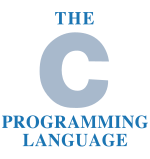
\includegraphics[scale=0.6]{images/c_prog.png}
\caption{C programnyelv logo.}
\end{figure}
A C programozási nyelvet Dennis Ritchi és Ken Thompson az '70es évek elején fejlesztette ki. Általános célú programozási nyelvek közé tartozik, ami annyit tesz, hogy nem tartalmaz olyan nyelvi elemeket, amik kifejezetten egy bizonyos szakterület számára hoztak létre ellentében a szakterület specifikus nyelvekkel.\\

Kifejlesztésének elsődleges célja az volt, hogy  UNIX operációs rendszert könnyen hordozhatóvá tegyék több számítógép között.
Ennek oka az volt hogy a UNIX assembly nyelven készült hordohatóság nagyon nehézkes volt, a szerzők először olyan magasszintű programozási nyelvet kerestek, ami alkalmas operációs rendszerek írására,emellett mégis egyszerű és hardware programozásra alkalmas. Mivel olyan nyelvet nem találtak, ami minden kritériumnak megfelelő lett volna, ezért Ritchie Thompson létrehozta a C programozási nyelvet.\cite{brian1978thec}\\

Ezáltal a UNIX lett az első olyan operációs rendszer,melynek jelentős része magasszintű programozási rendszerben íródott.\\

UNIX-on kívül később számos más operációs rendszerre készítettek C fordítót, idővel piacvezető programozási nyelvek egyike lett.\\

\noindent Továbbfejlesztett változata a C++, ami már a C objektum orientált bővítése.
\newpage
\noindent C nyelv legfontosabb jellemzői:
\begin{itemize}
\item struktúrált:\\
Lényege hogy minden feladat olyan kis feladatra legyen felosztva, amelyek egymással nincsenek átfedésben.
\item  szabványos:\\
Minden felületen van fordítóprogramja és a fordítás egységes szabvánnyal történik.
\end{itemize}

A klasszikus "Hello World!" C programnyelven a program neve: \texttt{pelda.c }.
\bigskip
\begin{cpp}
#include <stdio.h>
 main()
 {
 printf("Hello World!\n");
 } 
\end{cpp}
\bigskip
Ennek a példának a fordítása gcc fordítóval történik
\begin{cpp}
gcc -o pelda pelda.c
\end{cpp}
\bigskip
Futtatás:
\begin{cpp}
./pelda
\end{cpp}
\bigskip
Kimenet:
\begin{cpp}
Hello World!
\end{cpp}
\bigskip
\SubSection{GCC fordító}
\bigskip
\begin{figure}[h]
\centering

\includegraphics[scale=0.6]{images/gcc.png}
\caption{GCC logója.}
\end{figure}
\bigskip
GCC a GNU Compiler Collection rövidítése. Szabadon elérhető C fordító Linux rendszerre, de már létezik Windows-ra elkészített változata is (mingw-n keresztül). A mingw egy szoftveres portja a GNU Compiler Collection-nek windows felületre.\cite{gnu2003richard}

\SubSection{PCRE}

Perl Compatible Regular Expressions rövidítve PCRE egy olyan C nyelven írt könyvtár, ami reguláris kifejezés motort valósít meg. Philip Hazel 1997-ben kezdte el kifejleszteni. Szintaxtisa erősebb és rugalmasabb mint a POSIX reguláris kifejezéseknek.\cite{philip1997pcre}


\Section{OpenGL}
\begin{figure}[h]
\centering

\includegraphics[scale=0.6]{images/opengl_logo.jpg}
\caption{OpenGL logója.}
\end{figure}
\bigskip
Open Graphics Library rövidítve OpenGL egy részletesen kidolgozott szabvány,amit  Silicon Graphics amerikai cég fejlesztett ki az 1990-es években. Ez egy olyan programozásra alkalmas felület, amely felületen keresztül grafikus kártya kezelése és 3D programozása megvalósítható.\cite{mason1999opengl}

Maga a felület több ezer különböző függvényhívásból áll, melynek segítségével a programozó közvetlenül a grafikus kártya vezérlésével 3D alakzatokat rajzolhatnak ki és ezek megvalósítását szabályozhatják közben. Felhasználása elég széleskörben zajlik használják: tervezésben/gyártásban, VR (virtuális valóság) létrahozatalában és szimulátorok esetében is.\\

Támogatott platformok többet között Linux és Windows, de használják még mobiltelefonokon illetve játékkonzolon.\\

Az első verzió 1992. június 30-án jelent meg, azóta az OpenGL-t számos alkalommal bővítették új verzió kiadásával.\\

Mára a legújabb verzió az OpenGL 4.6 , ami hatákonyabb geometria feldolgozás és árnyékoló végrehajtást illetve térbeli irányoktól függő eltolást biztosít a felhasználónak korábbi verziókhoz képest.\cite{khronos1997opengl}





%\Section{Felhasznált technológiák}

